\documentclass{article}
\usepackage{caption}
\captionsetup{labelformat=empty}
\usepackage[utf8]{inputenc}
\usepackage{amsmath}
\usepackage{adjustbox}
\usepackage{tabu}
\usepackage{graphicx}
\usepackage{float}
\begin{document}
\section{Kullback-Leibler Divergence}
\subsection{Phonemes and Language Similarity}
\begin{itemize}
	\item[a)]
	A unified phoneme set is constructed from all the different language phonemes. The probability distribution of phonemes is calculated for each corpus with Lidstone smoothing where, $\alpha $= 1. Then 3 test cases are run for different unseen phonemes in different corpus. The probability of unseen phoneme '\$' is calculated in English and French corpus. The probability of another unseen phoneme '1' is calculated in Italian corpus. The test was successful, as in all cases it returns some very little probability value which is not zero. \:
	
	\item[b)]
	    From the bar chart below we can see that the distribution of phonemes in these 4 languages is not uniform at all. In each corpus frequency of some phonemes is much more than the others while there are also such phonemes which frequency is quite low than the remaining.  
		\begin{figure}[H]
            \centering
                \begin{minipage}{.55\textwidth}
                    \centering
                    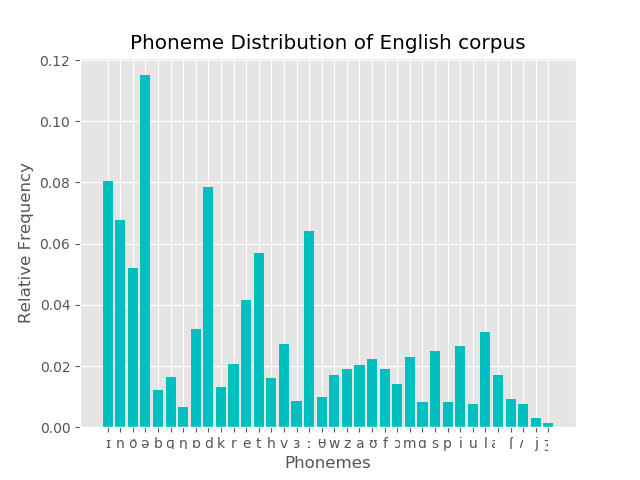
\includegraphics[keepaspectratio=true,scale=0.35]{English.png} 
                    \label{fig:prob1_6_2}
                \end{minipage}%
                \begin{minipage}{.5\textwidth}
                    \centering
                    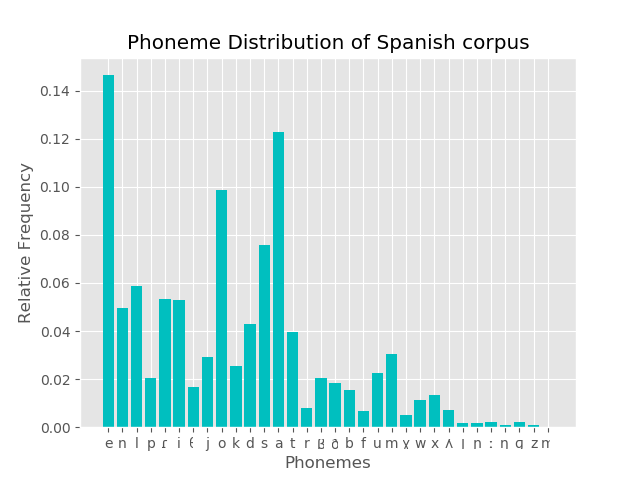
\includegraphics[keepaspectratio=true,scale=0.35]{Spanish.png}   
                    \label{fig:prob1_6_2}
                \end{minipage}
        \end{figure}
        \begin{figure}[H]
            \centering
                \begin{minipage}{.55\textwidth}
                    \centering
                    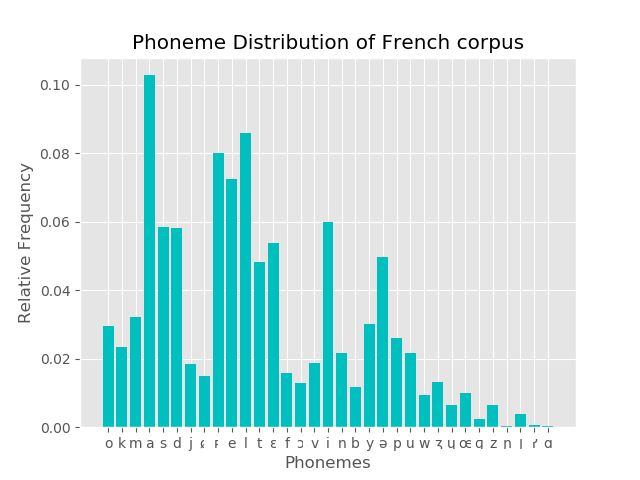
\includegraphics[keepaspectratio=true,scale=0.35]{French.png} 
                    \label{fig:prob1_6_2}
                \end{minipage}%
                \begin{minipage}{.5\textwidth}
                    \centering
                    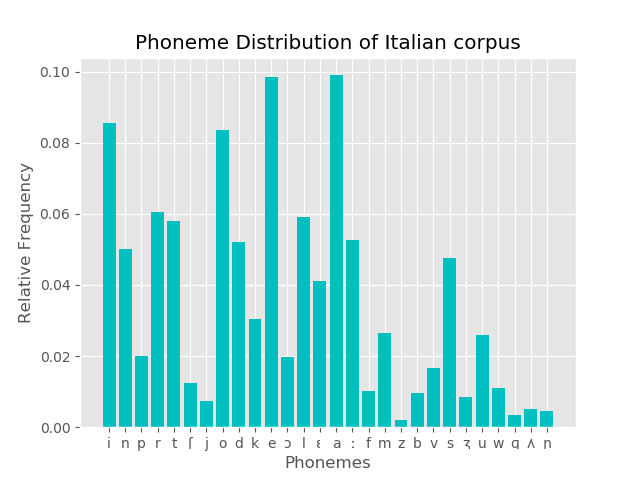
\includegraphics[keepaspectratio=true,scale=0.35]{Italian.png}   
                    \label{fig:prob1_6_2}
                \end{minipage}
        \end{figure}
        
    \item[c)]
    KL Divergence is computed for each corpus using the given formula which returns value in bits 
    \\\\\\
    \item[d)]  
        From the table below we can analyze the closeness of the phonemes of different language pair from their respective probability distribution. Similarity between same corpus is $100\%$ that is why in the table for the pair X*X the dissimilarity is 0. English phonemes are more closer to French than the others, Spanish are closer to Italian whereas, French is 1.6133101058269297 bits dissimilar to the Italian which is the closest from French to Italian. Italian is the closest to Spanish. However, we can not say vice versa. For example, we already analyzed that English phonemes are more closer to French than the others, but the opposite, French phonemes are more closer to English than the others does not hold. Because we already mentioned above that French phonemes have less dissimilarity with the Italian. So the value in the table English*French = 2.8261536675741477 bits and the value French*English = 2.430955266520877 bits do not match. Hence, the asymmetric property of the KL-divergence is justified.
        \begin{table}[ht]
            \centering
            \begin{tabular}{|c| c| c| c| c|}
                \hline 
                & English & Spanish & French & Italian \\ [0.5ex]
                \hline
                English & 0.0 & 3.4527781919333416 & 2.8261536675741477 & 3.187159871659876 \\
                \hline
                Spanish & 2.5457803433370376 & 0.0 & 1.3777115939406528 & 1.1271537967399006 \\
                \hline
                French & 2.430955266520877 & 2.296411824471215 & 0.0 & 1.6133101058269297 \\
                \hline
                Italian & 1.8778719008184728 &  1.0740189099914266 &  1.1985568480541147 &  0.0 \\ [1ex]
                \hline
            \end{tabular}
            \caption{\hspace*{4.0cm}Table: KL Divergence for all language pair}
        \end{table}
        \end{itemize}


\section{Language Models Evaluation}
\subsection{LM Evaluation - Perplexity}
\begin{itemize}
	\item[a)]
		$$peplaxity(\mathcal{V}) = 2^{-log(\frac{1}{M})}$$
	\item[b)]
		
\end{itemize}
\end{document}
